\documentclass[11pt]{article}
% Packages
\usepackage[utf8]{inputenc}
\usepackage[T1]{fontenc}
\usepackage[margin=1in]{geometry}
\usepackage{amsmath, amsthm, amsfonts, amssymb}
\usepackage{mathrsfs}           % \mathscr font.
\usepackage{setspace}
\usepackage[colorlinks=true,linkcolor=blue,citecolor=blue,urlcolor=blue,breaklinks]{hyperref}
\usepackage{graphicx}
\usepackage{booktabs}
\usepackage{xcolor}
\usepackage[style = authoryear, autocite=inline, doi=false,isbn=false,url=false]{biblatex}
\usepackage[sc]{titlesec} % make section headings \sffamily

% Header styling
% make headers \sffamily
\newpagestyle{main}[\sc]{
    \sethead{\thepage}{}{\sectiontitle}
    }
\pagestyle{main}
\usepackage{titling}
% make titling elements \sffamily
\pretitle{\begin{center}\sc \LARGE}
\preauthor{\begin{center}
            \large\sffamily \lineskip 0.5em%
            \begin{tabular}[t]{c}}
\predate{\begin{center}\sffamily\large}
\usepackage{abstract}
% make abstract title \sffamily
\renewcommand\abstractnamefont{\sffamily}
\titleformat{\section}[block]{\filcenter \Large \sc}{\thesection}{1em}{}
\usepackage{caption}
\captionsetup{font=sf, labelfont = bf}

% Define symbols and maths shortcuts
\DeclareRobustCommand{\bbone}{\text{\usefont{U}{bbold}{m}{n}1}}
\DeclareMathOperator{\EX}{\mathbb{E}} % expected value
\DeclareMathOperator{\V}{\mathbb{V}}
\DeclareMathOperator{\Prob}{\mathbb{P}}
\newcommand*{\trans}{^{\mathsf{T}}} %matrix transpose

\usepackage[long, nodayofweek]{datetime}
\usepackage[style = authoryear]{biblatex}

\addbibresource{../../literature/leapfrogging.bib}
\AtEveryBibitem{\clearfield{month}}
\newtheorem{assumption}{Assumption}
\usepackage{tikz}

\title{Party Competition between Regional Parties: A Framework for `Regional Outbidding'}
\author{Tobias Nowacki\thanks{Stanford University, Calif., USA. \texttt{tnowacki@stanford.edu}. With thanks to David Laitin and Apoorva Lal. This proposal is for a joint project with Apoorva Lal in mind.}}

% Begin Document
\begin{document}

\maketitle

\onehalfspacing

\section{Introduction}

This research proposal seeks to provide a first step towards a project explaining when and how parties that compete in a regional setting with distinct preferences that is nested in a larger, national democratic polity can take positions that are far away from the (regional) median voter. This puzzle is primarily motivated by the example of ethnic-nationalist parties in Catalonia, Scotland, Quebec or Flanders. All four of these cases have, at various points in their more recent history, seen ethnic-nationalist parties take extreme positions that threatened the breakup of the larger polity. This notion is also captured in Horowitz's idea of `ethnic outbidding' (but can be generalised to non-ethnic dimensions; hence the overall term `regional outbidding'). 

I propose a simple Downsian framework where a national (unionist) party competes both at the national and the regional level. Because it has to enter both elections with the same policy platform, but primarily cares about national elections, it will compete in the regional election with a fixed policy position that is removed from the regional median; this, in turn, gives rise to regional party competition that diverges from the median towards the other end. I sketch out multiple extensions of this model, such as policy-oriented parties and coalition formation mechanics.

Beyond simply illustrating a possible explanation for an empirical observation in Catalonia and elsewhere, this theoretical framework may be relevant in other ways. First, it is general enough that it can be applied to other policy dimensions as well: the crucial mechanic is a divergence in regional and national policy preferences, where the nation-wide electorate is tightly clustered towards one end of the dimension. Thus, the proposed framework may be useful to other literatures as well. Second, the specific application to ethnic-nationalist parties speaks to a well-developed literature on ethnic outbidding, which has been frequently observed but has seen few attempts to formalise the underlying mechanics. Third, extreme cases of divergence can result in the breakdown of either democratic institutions or the national polity altogether. Thus, this model may also offer a potential explanation for some cases of democratic breakdown.\footnote{Note that these are \textit{potential} areas for a contribution -- this short proposal alone certainly falls short of contributing to all three areas.}

\section{Literature and Motivation}

What explains the phenomenon of regional parties taking more extreme positions than the median voter of the respective electorate? This question is of particular interest when it comes to the dimension of ethnic nationalism or the distribution of power between the central polity and the region.

The idea of ethnic outbidding suggests that cross-ethnic or centrist coalitions cannot hold because its constituent ethnic parties are vulnerable to more extreme challengers; this results in a spiral of more and more extreme policy positions \parencite{Horowitz2000, Rabushka1972, Chandra2005}. Horowitz's contribution in particular sparked a large literature on ethnic politics; the term `ethnic outbidding' is widely used and referenced in relation to ethnicity-based parties. The role of elections in spurring ethnic conflict has also been considered (e.g., Cederman et al., 2012); however, this literature takes an \textit{ex post} perspective, analysing the likelihood of conflict after an election has taken place. Instead, the idea of ethnic outbidding suggests that there is something inherent about the \textit{ex ante} competition that leads to increasingly polarised policy platforms and, at worst, conflict and the breakdown of the polity.

Empirically, the phenomenon of increasingly more extreme ethnic parties has been widely observed, both in established democratic polities, such as Northern Ireland \parencite{Coakley2008, Mitchell2009, Moore2014,DeFazio2016} or Catalonia / Spain \parencite{Barrio2017}, as well as in developing countries (e.g., Sri Lanka \parencite{DeVotta2005}.

Yet, the mechanism that leads to increasingly polarised parties has not resulted in a large formal-theoretical literature. The `ethnic outbidding' mechanism is often only vaguely defined and rarely formalised. If we think of ethnicity as a continuous `policy dimension' with voters distributed across it, the classic Downsian model would predict convergence and a moderate stance. Furthermore, the threat from challengers implicitly assumes some form of entry mechanism that is not specified any clearer. Some attempts at a formalisation of the mechanism impose additional assumptions: in \textcite{Chandra2005}, for example, the depiction of Horowitz's theory requires that preferences are distributed fully dichotomously, doing away with a continuous distribution of voters. \parencite{Zuber2015} provide a theoretical framework that seeks to explain ethnic parties' positioning across two dimensions, and tests it using a novel dataset on national elections in European democracies. Yet, the question of what conditions induce ethnic outbidding, and what role the preference divergence between the national polity and the region has, remain unclear.

The model developed in this research proposal seeks to connect to this literature by offering a novel mechanism through which we can explain ethnic parties settling in a policy position that is more extreme than the median. Although the motivation primarily comes from regional parties in Europe (e.g., Catalonia), the underlying model can be applied to other policy areas, too. The crucial assumption here is that the national distribution of preferences is centred around one extreme of the policy dimension, whereas the regional one is distributed evenly or in a polarised fashion across both.

Another key question is whether the empirically observed process of polarisation is driven by changes in voters' preferences, or induced by party elites (and parties' changing policy positions). This research proposal seeks to explain ethnic polarisation as an outcome of the latter (for party-driven `ethnic outbidding' in Catalonia, see \textcite{Barrio2017}). That said, elite-driven polarisation may later induce a shift in voters' preferences, too \parencite[p. 291]{Horowitz2000}, which further contributes to the destabilisation of the polity. This endogenous relationship is worth noting on both theoretical grounds, as well as empirical, as it poses a significant challenge for any empirical strategy.

In summary, the idea for a contribution here is to offer a theory of multi-level elections, and how differences in the preference distribution between regional and national electorates can lead to divergence from the median voter position if multiple regional parties compete with each other. This can be applied to ethnicity or regional autonomy as examples of policy dimensions with strongly divergent preference distributions in the nation and the region; the regional competition may lead to parties advocating more extreme positions that may, in turn, threaten the unity of the polity and/or the democratic process. This theoretical framework thus intends to contribute to the literature on `ethnic outbidding', as well as explaining median voter divergence in regional elections more generally.

\section{Theoretical framework: baseline}

The general framework of the model is as follows: let there be two separate elections - one at the national level, and one at the regional level, with separate electorates (or we can assume that the regional electorate is a subset of the national one). There is a continuuous, unidimensional policy space $P \in [0, 1]$. Our main policy dimension of interest is ethnicity, or regional autonomy, but this could be substituted for any other policy dimension that exhibits the kinds of differences described below.\footnote{Ethnicity here would not be dichotomous, but a continuous dimension, e.g., voters can feel half-Spanish, half-Catalan. Perhaps thinking about it in a 'regional autonomy' way (secession all the way to centralised state) is a better way.} Let the dimension range from 0 to 1. The distribution of preferences between the two electorates differs: the national electorate is tightly clustered around one extreme (the unionist one), such that the median voter $\tilde{v}_N = 0.9$, whereas the regional electorate is either uniform or polarised around both extremes, and $\tilde{v}_R = 0.5$. For now, assume that the regional electorate is distributed uniformly with support $[0, 1]$.

For the purpose of the baseline model, let there be one national party, $N$, that competes in both the national and the regional election, and up to two regional parties, $R_1, R_2$, that only compete in the regional elections.\footnote{This is the baseline model -- for realism's sake, a more elaborate version of the model could include 2 national parties, yet they would still end up at the national median under these conditions.} Furthermore, I impose the following two assumptions:

\begin{assumption}
    The national party runs in both the national and the regional election, but cares about winning office in the national election; the regional parties only run in the regional election and care about winning in it.
\end{assumption}
\begin{assumption}
    The national party can only set one policy position, $p_N$, with which it has to run in both elections.
\end{assumption}

Assumption 1 can be rationalised as follows: the national party cares about the `bigger' office but in order to bolster its claim that it is a nation-wide party, it also has to run in all sub-national elections regardless of whether it anticipates to win or not. (This is not unlike the Spanish Partido Popular in Spain / Catalonia). Regional parties, on the other hand, by default only care about the regional election. Assumption 2 follows from a model of parties as uniform and centralised actors, which may be especially fitting for unionist parties that seek greater centralisation.

Finally, for the purpose of this baseline model, let all parties be office-seeking, that is, they want to maximise their vote share.

It follows from Assumption 1 that $N$ will determine its policy position ($p_N$) with respect to the national electorate; following the median voter theorem, it will always position itself at the national median, such that $p_N = \tilde{v}_N$. From this follows that $N$ will also compete in the regional elections with the same policy position, which, however, is far to the right of the \textit{regional} median. In the next subsections, I will show how regional parties react to this setting and how this may lead to two regional parties to the left of the median voter in equilibrium. This result may offer a first shot at a formal mechanism for elite-driven 'ethnic outbidding'.


\subsection{One regional party}

\begin{figure}[ht]
    \centering 
     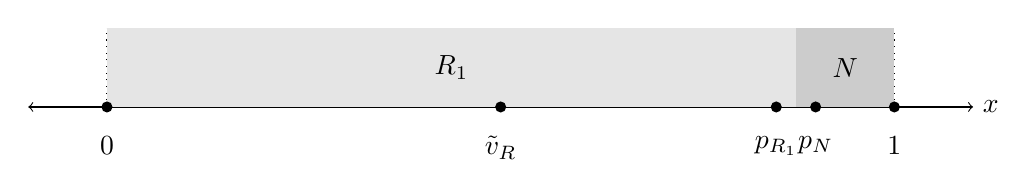
\begin{tikzpicture}
         % Axes
         \draw [<->] (-1,0) -- (11,0) node [right] {$x$};
         \draw [dotted] (0, 0) -- (0, 1);
         \draw [dotted] (10, 0) -- (10, 1);
         \draw [-] (0, 1) -- (10, 1);
         \fill [black!10] (0, 0) rectangle (8.75, 1);
         \draw (4.375, 0.5) node {$R_1$};
         \fill [black!20] (8.75, 0) rectangle (10, 1);
         \draw (9.375, 0.5) node {$N$};
         % Origin
         \node at (0,-.25) [below] {$0$};
         \node at (10, -.25) [below] {$1$};
         \node at (5, -.25) [below] {$\tilde{v}_R$};
         \node at (8.5, -.25) [below] {$p_{R_1}$};
         \node at (9, -.25) [below] {$p_{N}$};
         \coordinate (orig) at (0, 0);
         \coordinate (med)  at (5, 0);
         \coordinate (r1)   at (8.5, 0);
         \coordinate (N)    at (9, 0);
         \coordinate (end)  at (10, 0);
         \foreach \n in {orig, r1, med, N, end} \fill [black] (\n) circle (2pt);
     \end{tikzpicture}
     \caption{One national and one regional party; uniform distribution (regional electorate).} \label{fig:mod1}
 \end{figure}

 First, assume that there is only one regional party, $R_1$, that competes with $N$. 

 In equilibrium, it will position itself just to the left of $N$, and win the votes of everyone in the range from $[0, \frac{p_N + p_{R1}}{2}]$. $R_1$ has no incentive to move: moving further left would incur a vote loss towards $N$, and moving to the right of $N$ would leave them with a much smaller share of the distribution. Per assumption, $N$ cannot move its policy position. This is visualised in Figure \label{fig:mod1}. The resulting vote shares are $V_R = \frac{p_N + p_{R1}}{2}$ and $V_N = 1 - \frac{p_N + p_{R1}}{2}$.

As a consequence, the regional party positions itself close to the national party, and there is little issue competition on this dimension. Both are to the right of the regional median voter.\footnote{This is less problematic, because there is a reasonable argument that both the national and the regional party are close to the \textit{national} median voter. Whether that matters for evaluating the welfare outcome of this result for \textit{regional} elections is unclear.} It is likely that other divides (e.g., the classic left-right divide) are more salient in this scenario.

In practice, however, the regional party may position itself closer towards the median / the secessionist end, because of either inherent uncertainty or because of an intrinsic preference for a more autonomous policy. (see extensions to try and capture this. Another alternative is that they want to prevent any challengers from entering.) In either case, they will retain the majority of the vote share and thus capture office.\footnote{In the baseline model, the result suggests that they would be very close to $N$, purely because they'd rather win 90\% of the vote than `just' 60\%. That's not necessarily a plausible result, so the extensions may be crucial here.}

\subsection{Two regional parties}

\begin{figure}[ht]
    \centering 
     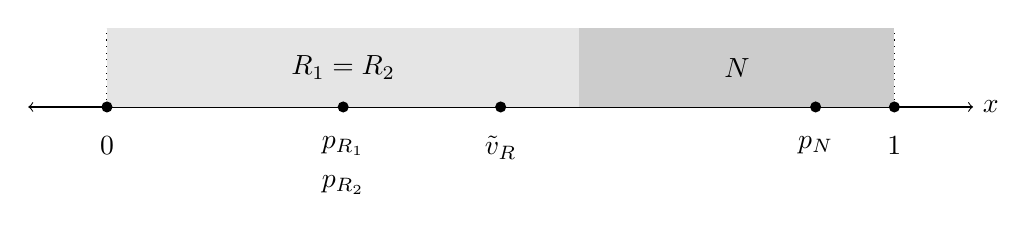
\begin{tikzpicture}
         % Axes
         \draw [<->] (-1,0) -- (11,0) node [right] {$x$};
         \draw [dotted] (0, 0) -- (0, 1);
         \draw [dotted] (10, 0) -- (10, 1);
         \draw [-] (0, 1) -- (10, 1);
         \fill [black!10] (0, 0) rectangle (6, 1);
         \draw (3, 0.5) node {$R_1 = R_2$};
         \fill [black!20] (6, 0) rectangle (10, 1);
         \draw (8, 0.5) node {$N$};
         % Origin
         \node at (0,-.25) [below] {$0$};
         \node at (5,-.25) [below] {$\tilde{v}_R$};
         \node at (10, -.25) [below] {$1$};
         \node at (3, -.25) [below] {$p_{R_1}$};
         \node at (3, -.75) [below] {$p_{R_2}$};
         \node at (9, -.25) [below] {$p_{N}$};
         \coordinate (orig) at (0, 0);
         \coordinate (med)  at (5, 0);
         \coordinate (r1)   at (3, 0);
         \coordinate (N)    at (9, 0);
         \coordinate (end)  at (10, 0);
         \foreach \n in {orig, r1, med, N, end} \fill [black] (\n) circle (2pt);
     \end{tikzpicture}
     \caption{One national and two regional parties; uniform distribution (regional electorate).} \label{fig:mod1}
 \end{figure}

Next, suppose that there are two regional parties, $R_1$ and $R_2$ that compete together with $N$. I keep the assumption of uniformly distributed voters for now, before discussing a more general case in the next subsection.

As before, $N$ keeps its policy position fixed at $p_N = \tilde{v}_N$. In equilibrium, both regional parties position themselves at $p_N / 3$, such that they split the voters in the range $[0, 2 p_N/3]$ between them. Their vote shares are thus $V_{R1} = V_{R2} = p_N / 3$, whereas $N$ receives $V_N = 1 - \frac{2}{3} p_N$. Here, neither regional party has an incentive to move. Moving leftwards would only decrease their vote share to below $p_N / 3$; moving rightwards they would only swap votes they would gain from $N$ with those lost to the other regional party. The best they could do by moving rightwards is to position themselves at $2/3 p_N$, which would see them gain the same vote share again; however, in this case, $R_2$ could move closer again in order to optimise their vote share (thus, $(p_N / 3, 2 p_N/3, p_N) $ cannot be an equilibrium). Finally, there is no incentive to move to $p_N$: the split vote share with $N$ would be smaller than the split vote share with $R_2$. Note that this imposes the constraint $p_N \geq 0.75$ for this to be an equilibrium.\footnote{The vote share that $R$ gets in equilibrium must be greater than the vote share it would get if it were to share its policy position with $N$ instead, that is, the inequality $v_R \geq V_N / 2$ or $\frac{1}{3} p_N \geq (1 - \frac{2}{3} p_N) / 2$ must hold. This simplifies to $p_N \geq 0.75$.}

One remaining comparative static is the position of $p_N$ within the constraint. The closer to the median voter $N$ is, the smaller is the mass of voters in $[0, p_N]$. Consequently, since the regional parties will position themselves at $p_N / 3$, this position will be further left (and further away from the median), the smaller (i.e., closer to the median) $p_N$ is.

This result shows how the competition between the two regional parties can drive them to take on more extreme policy positions that are to the left of the regional median voter, and certainly far to the left of the national median voter. This captures a possible mechanism for `ethnic outbidding': given the fixed policy position of the national party, and their proximity to unionist-minded voters, the two regional parties compete for the attachment of the regional ethnicity instead, thus forgoing the compromise position between the two (i.e., the median voter).

\subsection{Two regional parties, polarised distribution}

The result from the previous subsection can be stated more generally, as long as the underlying distribution of voters is symmetric around the median voter, and the density is weakly increasing on either side of the median voter.\footnote{With `humps' in the distribution, the equilibrium may not work, as parties may take up more than 1/3 of the share if it's tightly clustered together -- hence the weakly increasing density condition.} Under these assumptions, the distribution of voters can be polarised towards the extremes.\footnote{The constraint on $p_N$ discussed in footnote 5 still holds in some form, but with a non-uniform distribution I would need to express it more generally.}

Let $f(x)$ denote the pdf of voters with support over the policy dimension, $x \in [0, 1]$; let $F(x)$ denote the cdf, and $F^{-1}(x)$ the inverse of the cdf or the quantile function.

The equilibrium can be restated in general terms:

\begin{align*}
    p_{R1} = p_{R2} & = F^{-1}\Big(\frac{F(p_N)}{3}\Big) \\
    p_N & = \tilde{v}_N
\end{align*}

The regional parties position themselves such that they are at the first tercile of the voter mass in $[0, p_N]$. This remains an equilibrium for the regional parties because by moving leftwards, they would get less than that tercile of voters; by moving rightwards, they cannot get more than a tercile either (the weak increase and symmetry assumptions ensure that); this is true of the uniform distribution already, and any other distribution considered here would be more polarised, such that by moving closer towards the centre I would give up more voters to the left than I would gain in the centre.

The corresponding vote shares are:

\begin{align*}
    V_{R1} = V_{R2} & = \frac{1}{2} F(\frac{p_{R1} + p_N}{2}) \\
    V_N & = 1 - F(\frac{p_{R1} + p_N}{2})
\end{align*}

Note that these vote shares may be $v_{R1} = v_{R2} \neq \frac{1}{3} F(p_N)$ if we depart from the uniform distribution (because the second tercile point may not necessarily be equidistant from $p_R$ and $p_N$).

As the distribution becomes more polarised, $p_R$ move further towards the extreme. This is because the result suggests they locate themselves at the point of the first tercile of the voters between $[0, p_N$]; with a more polarised distribution, that tercile point moves closer towards the extreme.

\begin{figure}
    \centering
    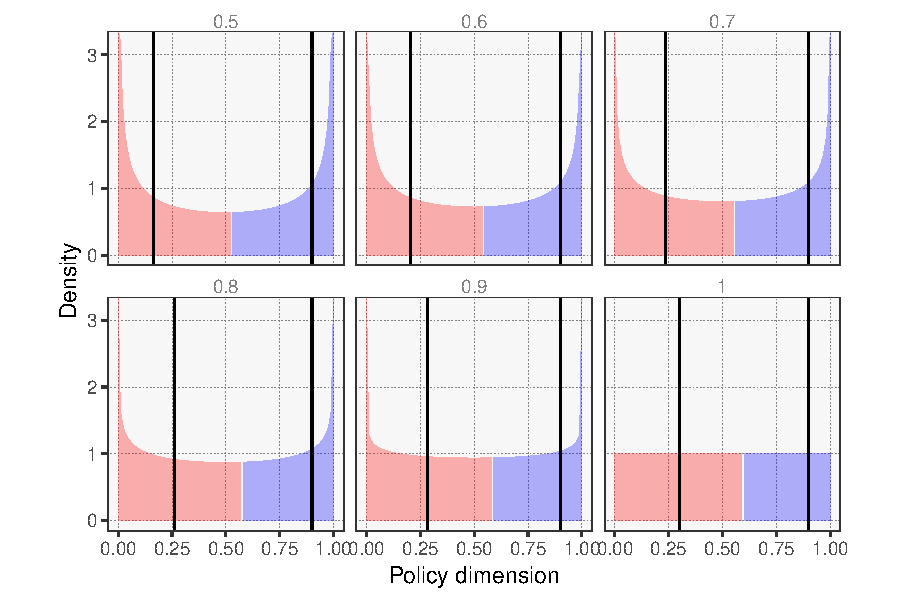
\includegraphics{../../output/polarisation.pdf}
    \caption{Equilibrium positions under different parameter values for Beta distribution.}
    \label{fig:betadist}
\end{figure}

One way to model a symmetric, polarised distribution is the beta distribution:

\begin{equation*}
    \frac{x^{\alpha - 1}(1 - x)^{\beta -1}}{B(\alpha, \beta)}
\end{equation*}

When $\alpha = \beta = 1$, this collapses into a uniform distribution; when $0 < \alpha = \beta < 1$, the beta distribution is symmetric around $0.5$ and adds weight to the extremes. Figure~\ref{fig:betadist} plots the distribution of voters, parties' policy points in equilibrium, and their share of voters, for different parameters ($\alpha = \beta \in [0.5, 1]$) of the beta distribution. This illustrates the result that, as the distribution becomes more polarised, the regional parties' equilibrium shifts towards the extreme and divergence from the median increases.

\subsection{Summary and key results}

The model yields the following results so far:
\begin{itemize}
    \item With a national party's fixed policy position, and a strong divergence between regional and national preferences, two regional parties will take policy positions that are more extreme than the median;
    \item When polarisation increases, the regional parties will take more extreme positions;
    \item The more accommodating the national party is, the more extreme will the positions of the regional parties be.
\end{itemize}



\section{Extensions and challenges}

\subsection{Model extensions}

\textsc{Policy-oriented parties.} One possible extension is to model the regional parties as caring about both office winning \textit{and} and a policy ideal point such as $x = 0$ (which could be independence in the ethnicity example). The expectation here would be that this would distort the regional party's policy platform even further from the median, as the ideal point pulls them even further towards the left.\footnote{In the case with only one regional party, this example is very simple: rather than positioning itself immediately to the left of $N$, it would go as far left as long as it still commands a majority of the vote. If $N$ = 0.9 and the ideal point is still 0, then the optimal policy platform would be $p_R = 0.1 + \epsilon$.}

\textsc{Coalition formation and electoral system.} The model with three parties would suggest that none of them capture a majority of the seats. This necessarily introduces a second stage to the game, where parties bargain and form a coalition. If, in equilibrium, the two regional parties have the same policy platform, it would make sense for them to form a coalition. Suppose, as a thought, that they both also have their ideal policy point at $x = 0$. I would have to model explicity benefits to office and the coalition formation stage of the game, but there could be a situation where one of the parties positions itself strategically at $x = 0$ in order to pull the weighted average of the coalition with their more centrist partner further towards the extreme.

Another extension that gives the game more structure is a distinction between PR and plurality. Implicitly, this discussion has so far assumed PR - but it would be interesting to see if there was a change in results if parties had to appeal to multiple districts (with heterogeneous median voters) under plurality instead.

\textsc{Dynamics.} Another idea for an extension is the introduction of dynamics and entry/exit of parties. Using the set-up with only one national and one regional party as a baseline, under what conditions would a challenging regional party decide to enter? It would be interesting to model the outbidding process dynamically (i.e. with parties leapfrogging each other subsequently to arrive at more extreme positions), though I am not sure if this can be reconciled easily with the simple equilibrium results from the baseline model.

\subsection{Empirical extension \& Application}

Yet another challenge for this project is the empirical application of this model. Because of the relative scarcity of distinct ethnicities in peripheral regions in established democracies, a large-N analysis may be difficult. Recent new datasets include EPAC \parencite{Szocsik2015}, with expert survey data on ethnic-nationalist positions in 22 European democracies, and the Regional Manifestos Project, which measures party positions through manifesto text analysis \parencite{Alonso2013}. These new data can be used to estimate parties' policy positions and test the predictions of the model (although causal identification is near impossible in this context). In addition, case studies of the classic cases (Catalonia, Scotland, Quebec) may serve to illustrate and underpin the proposed model.

In particular, at a first glance, these cases do exhibit some of the features in this model: 
\begin{itemize}
    \item two parties `outbidding' each other in Catalonia (ERC and Convergència);
    \item Shifts in the national party positions on regional autonomy in Scotland (Labour introducing devolution in 1997);
    \item The split in the Quebecois nationalist movement in 2012, going from one regional party to two.
\end{itemize}

\section{Conclusion}

This research proposal suggested a new theoretical framework that explains why regional or ethnic parties take policy positions that strongly diverge from the median, and, in the worst case, can lead to conflict and democratic breakdown. The model applies to cases where the regional distribution of preferences along a policy dimension differs significantly from the national one. Because the national party primarily cares about nationwide elections, its policy position will be towards one extreme of the regional median voter; if two regional parties compete, they will locate themselves towards the other extreme. This becomes more acute the more polarised the distribution of preferences in the region is. The model can be primarily applied to cases of `ethnic outbidding', and speaks to a large literature about this mechanism (cf. \textcite{Horowitz2000}), but may also be relevant for other policy dimensions.

\renewcommand*{\mkbibnamefamily}[1]{\textsc{\textbf{#1}}}
\renewcommand*{\mkbibnamegiven}[1]{\textsc{#1}}
\printbibliography

\end{document}
